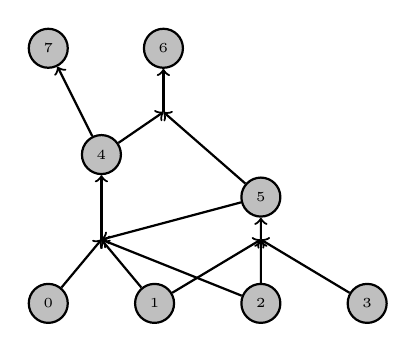
\begin{tikzpicture}[scale=0.45, yscale=1.2, thick] % , baseline = -3.5pt


	\node [circle, draw, thick, fill=gray!50] (T1) at (0,0) {\tiny $\lneuronof{0}$};
	\node [circle, draw, thick, fill=gray!50] (T2) at (3,0) {\tiny $\lneuronof{1}$};
	\node [circle, draw, thick, fill=gray!50] (T3) at (6,0) {\tiny $\lneuronof{2}$};
	\node [circle, draw, thick, fill=gray!50] (T4) at (9,0) {\tiny $\lneuronof{3}$};
	
	\node [circle, draw, thick, fill=gray!50] (ph) at (1.5,3.5) {\tiny $\lneuronof{4}$};
	\node [circle, draw, thick, fill=gray!50] (ph2) at (6,2.5) {\tiny  $\lneuronof{5}$};	
	
	\node [circle, draw, thick, fill=gray!50] (head) at (3.25,6) {\tiny $\lneuronof{6}$};
	\node [circle, draw, thick, fill=gray!50] (head2) at (0,6) {\tiny $\lneuronof{7}$};

	\draw[->] (ph) -- (head2);

	\coordinate (S3) at (3.25,4.5);
	\draw[->] (S3) -- (head);
	%\draw [->] (sel3) -- (S3);
	\draw [->] (ph2) -- (S3);
	\draw [->] (ph) -- (S3);
	
	\coordinate (S1) at (1.5,1.5);
	\draw[->] (S1) -- (ph);
	\draw [->] (T1) -- (S1);
	\draw [->] (T2) -- (S1);
	\draw [->] (T3) -- (S1);	
	\draw [->] (ph2) -- (S1);	
	
	\coordinate (S2) at (6,1.5);
	\draw[->] (S2) -- (ph2);
	%\draw [->] (sel) -- (S1);		
	%\draw [->] (sel2) -- (S2);

	\draw [->] (T2) -- (S2);
	\draw [->] (T3) -- (S2);	

	\draw [->] (T4) -- (S2);



\end{tikzpicture}